\documentclass{article} % For LaTeX2e
\usepackage[classfont=slant,langfont=caps,basic]{complexity}
\usepackage{amssymb}
\usepackage{amsmath}
\usepackage{amsthm}
\usepackage{multirow}
\usepackage{graphicx}
\usepackage[scriptsize,tight]{subfigure}
\usepackage{hyperref}
\usepackage[all]{hypcap}
\usepackage{xspace}
\usepackage{wrapfig}
\usepackage{algorithm}
\usepackage{algorithmic}
\usepackage{nips12submit_e,times}
%\documentstyle[nips12submit_09,times,art10]{article} % For LaTeX 2.09


\title{Bayesian Hierarchical Reinforcement Learning}

\author{
Feng Cao\\
Department of Electrical Engineering and Computer Science\\
Case Western Reserve University\\
Cleveland, OH 44106 \\
\texttt{fxc100@case.edu} \\
\And
Soumya Ray \\
Department of Electrical Engineering and Computer Science \\
Case Western Reserve University\\
Cleveland, OH 44106 \\
\texttt{sray@case.edu} \\
}

% The \author macro works with any number of authors. There are two commands
% used to separate the names and addresses of multiple authors: \And and \AND.
%
% Using \And between authors leaves it to \LaTeX{} to determine where to break
% the lines. Using \AND forces a linebreak at that point. So, if \LaTeX{}
% puts 3 of 4 authors names on the first line, and the last on the second
% line, try using \AND instead of \And before the third author name.

\newcommand{\fix}{\marginpar{FIX}}
\newcommand{\new}{\marginpar{NEW}}

%\nipsfinalcopy % Uncomment for camera-ready version

\begin{document}

\maketitle

\begin{abstract}
We describe an approach to incorporating Bayesian priors in the {\sc
maxq} framework for hierarchical reinforcement learning (HRL). We
define priors on the primitive environment model and on task
pseudo-rewards. Since models for composite tasks can be complex, we
use a mixed model-based/model-free learning approach to find an
optimal hierarchical policy. We show empirically that (i) our approach
results in improved convergence over non-Bayesian baselines, given
sensible priors, (ii) using both task hierarchies and Bayesian priors
is better than either alone, (iii) taking advantage of the task
hierarchy significantly reduces the computational cost of Bayesian
reinforcement learning and (iv) in this framework, task pseudo-rewards
can be learned instead of being manually specified, leading to
automatic learning of hierarchically optimal rather than recursively
optimal policies.
\end{abstract}

\section{Introduction}
\label{sec:intro}

Reinforcement learning (RL) is a well known framework that formalizes
decision making in unknown, uncertain environments. RL agents learn
policies that map environment states to available actions while
optimizing some measure of long-term utility. While various algorithms
have been developed for RL~\cite{suttbarto}, and applied successfully
to a variety of tasks~\cite{kaelbling.jair96}, the standard RL setting
suffers from at least two drawbacks. First, it is difficult to scale
standard RL approaches to large state spaces with many factors (the
well-known ``curse of dimensionality''). Second, vanilla RL approaches
do not incorporate prior knowledge about the environment and good
policies.

{\em Hierarchical reinforcement learning} (HRL)~\cite{barto.deds03}
attempts to address the scaling problem by simplifying the overall
decision making problem in different ways. For example, one approach
introduces macro-operators for sequences of primitive actions. 
Planning at the level of these operators may result in
simpler policies~\cite{stolle.book02}. Another idea is to decompose
the task's overall value function, for example by
defining task hierarchies~\cite{d-hrl-00} or partial programs with
choice points~\cite{alisp}. The structure of the decomposition
provides several benefits: first, for the ``higher level'' subtasks,
policies are defined by calling ``lower level'' subtasks (which may
themselves be quite complex); as a result policies for higher level
subtasks may be expressed compactly. Second, a task hierarchy or
partial program can impose constraints on the space of policies by
encoding knowledge about the structure of good policies and thereby
reduce the search space. Third, learning within subtasks allows {\em
  state abstraction}, that is, some state variables can be ignored
because they do not affect the policy within that subtask. This also
simplifies the learning problem.

While HRL attempts to address the scalability issue, it does not take
into account probabilistic prior knowledge the agent may have about
the task. For example, the agent may have some idea about where
high/low utility states may be located and what their utilities may
be, or some idea about the approximate shape of the value function or
policy. {\em Bayesian reinforcement learning} addresses this issue by
incorporating priors on models~\cite{dearden.uai99}, value
functions~\cite{Dearden98, Engel03} or
policies~\cite{Ghavamzadeh07bayesianpolicy}.
Specifying good priors leads to many benefits, including initial good
policies, directed exploration towards regions of uncertainty, and
faster convergence to the optimal policy.

In our work, we propose an approach that incorporates Bayesian priors
in hierarchical reinforcement learning. We use the {\sc maxq}
framework~\cite{d-hrl-00}, that decomposes the overall task
into subtasks so that value functions of the individual subtasks can
be combined to recover the value function of the overall task. We
extend this framework by incorporating priors on the primitive
environment model and on task pseudo-rewards. In order to avoid
building models for composite tasks (which can be very complex), we
adopt a mixed model-based/model-free learning approach.  We
empirically evaluate our algorithm to understand the effect of the
priors in addition to the task hierarchy. Our experiments indicate
that: (i) taking advantage of probabilistic prior knowledge can lead
to faster convergence, even for HRL, (ii) task hierarchies and
Bayesian priors can be complementary sources of information, and using
both sources is better than either alone, (iii) taking advantage of
the task hierarchy can reduce the computational cost of Bayesian RL,
which generally tends to be very high, and (iv) task pseudo-rewards
can be learned instead of being manually specified, leading to
automatic learning of hierarchically optimal rather than recursively
optimal policies. In this way Bayesian RL and HRL are synergistic:
Bayesian RL improves convergence of HRL and can learn hierarchy
parameters, while HRL can reduce the computational cost of Bayesian
RL.

Our work assumes the probabilistic priors to be given in advance and
focuses on learning with them. Other work has addressed the issue of
obtaining these priors. For example, one source of prior information
is multi-task reinforcement learning~\cite{Lazaric_bayesianmulti-task,
icml2007}, where an agent uses the solutions of previous RL tasks to
build priors over models or policies for future tasks. We also assume
the task hierarchy is given. Other work has explored learning {\sc
maxq} hierarchies in different settings~\cite{mehta.icml08}.

\section{Background and Related Work}
\label{sec:relwork}

% In this section, we describe  {\sc maxq} and Bayesian model-based reinforcement
% learning.

In the {\sc maxq} framework, each composite subtask $T_i$ defines a
semi-Markov decision process  with parameters $\langle
S_i,X_i,C_i,G_i \rangle$. $S_i$ is a predicate that defines the set of
``non-terminal'' states for $T_i$, where $T_i$ may be called by its
parent. $G_i$ is a predicate that defines a set of ``goal'' states for
$T_i$. 
% Thus {\sc maxq} tries to learn a value function (or policy) for $T_i$
% that takes it from any $S_i$ to any $G_i$. 
The actions available
within $T_i$ are described by the set of ``child tasks'' $C_i$.
Finally, $X_i$ denotes the set of ``relevant state variables'' for
$T_i$. 
% These variables parametrize the value function (or
% policy) that MAXQ learns for $T_i$.  
Often, we unify  $S_i$ and (the negation of) $G_i$ into a single
``termination'' predicate, $P_i$. A (state, action, next-state)
$(s,a,s')$ triple where $P_i(s)$ is false, $P_i(s')$ is true, $a \in
C_i$, and the transition probability $P(s'|s,a)>0$ is called an {\em
  exit} of the subtask $T_i$. A pseudo-reward function
$\tilde{R}(s,a)$ can be defined over exits to express preferences over
the possible exits of a subtask. 
% Pseudo-rewards are often used to
% provide ``contextual'' information to a subtask about the behavior of
% the rest of the task hierarchy.

A subtask can be invoked in any state $s$ where $P_i(s)$ is false, and
it terminates when an exit causes $P_i(s')$ to become true.  The set
$S_i$ is defined using a projection function that maps a world state
to an abstract state defined by a subset of the state variables. %  If
% the abstraction function is \textit{safe}, it will only merge the
% world states that have the same value function into an abstracted
% state.
%   A {\em local policy} for the subtask $T_i$ is a mapping from
% the states $S_i$ to $C_i$.
  A hierarchical policy $\pi$ for the
overall task is an assignment of a local policy to each SMDP $T_i$.  A
\textit{hierarchically optimal policy} is a 
hierarchical policy that has the maximum expected reward.  A
hierarchical policy is said to be \textit{recursively optimal} if the
local policy for each subtask is optimal given that all its subtask
policies are optimal.  Recursively optimal policies can be obtained by
fixing all pseudo-rewards to zero. Given a task graph,
model-free~\cite{d-hrl-00} or model-based~\cite{rmax-maxq} methods can
be used to learn value functions for each task-subtask pair.
% , and used
% to determine the hierarchical policy (which subtask to call at each
% level for each state). 
In the model-free method, a policy is produced
by maintaining a value and a {\em completion} function for each
subtask. For a task $i$, the value $V(a,s)$ denotes the expected value
of calling child task $a$ in state $s$. This is (recursively)
estimated as the expected reward obtained while executing
$a$. The completion function $C(i,s,a)$ denotes the expected
 reward obtained while {\em completing} $i$ after having
called $a$ in $s$. The central idea behind {\sc maxq} is that the
value of $i$, $V(i,s)$, can be (recursively) decomposed in terms of
$V(a,s)$ and $C(i,s,a)$. 
% In fact, by maintaining and updating
% $C(i,s,a)$ and $V(a,s)$ for primitive $a$, it is possible to
% reconstruct $V(i,s)$ for any $i$ and so construct a hierarchical
% policy.

Bayesian reinforcement learning methods incorporate probabilistic
prior knowledge on models~\cite{dearden.uai99}, value
functions~\cite{Dearden98,Engel03},
policies~\cite{Ghavamzadeh07bayesianpolicy} or
combinations~\cite{ghavamzadeh:icml07}. One Bayesian model-based
RL algorithm proceeds as follows. At each step, a distribution over
model parameters is maintained.  At each step, a model is sampled from this distribution
(Thompson sampling~\cite{Thompson, Strens}). This model is then solved
and actions are taken according to the policy obtained. This yields
observations about the environment model. These are used
to update the parameters of the current distribution to create a
posterior distribution over models. This procedure is then iterated to convergence.
% As more observations are obtained, the posterior distribution is
% refined to focus around the true environment model, and the policy
% asymptotically converges to the optimal policy for this model.
Variations of this idea have been investigated; for
example, some work converts the distribution over models to an
empirical distribution over $Q$-functions, and produces policies by
sampling from this distribution instead~\cite{dearden.uai99}.

Relatively little work exists that attempts to incorporate
probabilistic priors into HRL. We have found one preliminary
attempt~\cite{Zhao-bhrl-2010}. This work builds on the {\sc
  rmax+maxq}~\cite{rmax-maxq} method, which extends {\sc
  rmax}~\cite{Brafman01r-max} to {\sc maxq} by maintaining models for
each subtask and performing {\sc rmax}-style exploration in each. The
Bayesian approach adds priors onto each subtask model and performs
(separate) Bayesian model-based learning for each
subtask.~\footnote{While we believe this description is accurate,
  unfortunately, due to language issues and some missing technical and
  experimental details in the cited article, we have been unable to
  replicate this work.} In our approach, we do not construct models
for subtasks, which can be very complex in general.  Instead, we only
maintain distributions over primitive actions, and use a mixed
model-based/model-free learning algorithm that naturally integrates
into the standard {\sc maxq} learning algorithm. 

\section{Bayesian {\sc MAXQ} Algorithm}
\label{sec:algo}

In this section, we describe our approach to incorporating
probabilistic priors into {\sc maxq}. We use priors over 
primitive models and pseudo-rewards. As we explain below,
pseudo-rewards are value functions; thus our approach
uses priors both on models and value functions. While such an
integration may not be needed for standard Bayesian RL, it appears
naturally in our setting.

We first describe our approach to incorporating priors on environment
models alone (assuming pseudo-rewards are fixed). We do this following
the Bayesian model-based RL framework. At each step we have a
distribution over environment models (initially the prior). The
algorithm has two main subroutines: the main {\sc Bayesian\_MAXQ}
routine (Algorithm~\ref{alg:bmaxq}) and an auxiliary {\sc
Recompute\_value} routine (Algorithm~\ref{alg:recompvalue}). In this
description, the value $V$ and completion $C$ functions are assumed to
be global.
% The main {\sc
%   Bayesian\_MAXQ} routine interacts with the world using the current
% value estimates and updates the posterior over the environment models.
% Every $k$ steps, it calls the {\sc Recompute\_value} function to 
% resample a model from the posterior and recomputes the
% value and completion functions to reflect this new model. As in
% Bayesian model-based RL, this continues until the
% hierarchical policy converges. 
At the start of each episode, the {\sc Bayesian\_MAXQ} routine is
called with the $Root$ task and the initial state for the current
episode. The {\sc maxq} execution protocol is then followed, where
each task chooses an action based on its current value function
(initially random). When a primitive action is reached and executed,
it updates the posterior over model parameters
(Line~\ref{line:update}) and its own value estimate (which is just the
reward function for primitive actions). When a task exits and returns
to its parent, the parent subsequently updates its completion function
based on the current estimates of the value of the exit state
(Lines~\ref{line:comp1}~and~\ref{line:comp2}). Note that in {\sc
  maxq}, the value function of a composite task can be (recursively)
computed using the completion functions of subtasks and the rewards
obtained by executing primitive actions, so we do not need to
separately store or update the value functions (except for the
primitive actions where the value function is the reward). Finally,
each primitive action maintains a count of how many times it has been
executed and each composite task maintains a count of how many child
actions have been taken.

When $k$ (an algorithm parameter) steps have been executed in a
composite task, {\sc Bayesian\_MAXQ} calls {\sc Recompute\_value} to
re-estimate the value and completion functions (the check on $k$ is
shown in {\sc Recompute\_value}, Line~\ref{line:checkk}). When
activated, this function recursively re-estimates the value/completion
functions for all subtasks of the current task. At the level of a
primitive action, this simply involves resampling the reward and
transition parameters from the current posterior over models. For a
composite task, we use the {\sc maxq-q} algorithm (Table 4
in~\cite{d-hrl-00}). We run this algorithm for $Sim$ episodes,
starting with the current subtask as the root, with the current
pseudo-reward estimates (we explain below how these are obtained).
This algorithm recursively updates the completion function of the task
graph below the current task. Note that in this step, the subtasks
with primitive actions use model-based updates. That is, when a
primitive action is ``executed'' in such tasks, the currently sampled
transition function (part of $\Theta$ in Line~\ref{line:sample}) is
used to find the next state, and then the associated reward is used to
update the completion function. This is similar to
Lines~\ref{line:recursive},~\ref{line:comp1} and \ref{line:comp2} in
{\sc Bayesian\_maxq}, except that it uses the sampled model $\Theta$
instead of the real environment. After {\sc Recompute\_value}
terminates, a new set of value/completion functions are available for
{\sc Bayesian\_maxq} to use to select actions.

\begin{algorithm}[t]
\caption{{\sc Bayesian\_maxq}} \label{alg:bmaxq}
\begin{algorithmic}[1]
\REQUIRE Task $i$, State $s$, Update Interval $k$, Simulation Episodes $Sim$
\ENSURE Next state $s'$, steps taken $N$, cumulative reward $CR$
\IF{$i$ is primitive}    %%%% if primitive
\STATE Execute $i$, observe $r$, $s'$
\STATE Update current posterior parameters $\Psi$ using ($s$, $i$, $r$, $s'$)~\label{line:update}
\STATE Update current value estimate: $V(i,s) \leftarrow (1-\alpha)\cdot V(i,s)+\alpha\cdot r$
\STATE $Count(i) \leftarrow Count(i)+1$
\RETURN $(s', 1, r)$
\ELSE               %%%% composite
\STATE $N \leftarrow 0$, $CR \leftarrow 0$, $taskStack \leftarrow Stack()$\COMMENT{$i$ is composite}
%\STATE $CR \leftarrow 0$ 
%\STATE $taskStack \leftarrow Stack()$
\WHILE {$i$ is not terminated} 
\STATE {\sc Recompute\_value}$(i, k, Sim)$
\STATE $a\leftarrow \epsilon$-greedy action from $V(i, s)$
\STATE $\langle s', N_a, cr\rangle \leftarrow$ {\sc Bayesian\_maxq}($a$, $s$) ~\label{line:recursive}
\STATE $taskStack.push(\langle a, s', N_a, cr \rangle)$    
\STATE $a^*_{s'}\leftarrow \arg\max_{a'}\bigl[\tilde{C}(i,s',a')+V(a',s')\bigr]$ ~\label{line:comp1}
\STATE $C(i,s,a)\leftarrow(1-\alpha)\cdot C(i,s,a) + \alpha\cdot \gamma^{N_a}\bigl[C(i,s',a^*_{s'})+V(a^*_{s'},s') \bigr]$~\label{line:comp2}
\STATE $\tilde{C}(i,s,a)\leftarrow(1-\alpha)\cdot \tilde{C}(i,s,a) + \alpha\cdot \gamma^{N_a}\bigl[\tilde{R}(i, s')+\tilde{C}(i,s',a^*_{s'})+V(a^*_{s'},s') \bigr]$
%\STATE $s\leftarrow s'$
\STATE $s\leftarrow s'$, $CR \leftarrow CR+\gamma^N\cdot cr$, $N\leftarrow N+N_a$, $Count(i) \leftarrow Count(i)+1$
%\STATE $N\leftarrow N+N_a$
%\STATE $Count(i) \leftarrow Count(i)+1$
\ENDWHILE
\STATE {\sc Update\_pseudo\_reward}($taskStack$, $\tilde{R}(i, s')$)
\RETURN $(s', N, CR)$
\ENDIF
\end{algorithmic}
%\vspace{-0.2in}
\end{algorithm} 


%%%%%%%%%%%%%%%%%%%%%%%%%%%%%%%%%%%
%%%%  Compute-policy
%%%%%%%%%%%%%%%%%%%%%%%%%%%%%%%%%%%
\begin{algorithm}[t]
\caption{{\sc Recompute\_value}} \label{alg:recompvalue}
\begin{algorithmic}[1]
\REQUIRE Task $i$, Update Interval $k$, Simulation Episodes $Sim$
\ENSURE Recomputed value and completion functions for the task graph below and including $i$
\IF{$Count(i) < k$}
\RETURN~\label{line:checkk}
\ENDIF
\IF{$i$ is primitive}  
\STATE Sample new transition and reward parameters $\Theta$ from
current posterior $\Psi$~\label{line:sample}
\ELSE
\FORALL {child tasks $a$ of $i$}
\STATE {\sc Recompute\_value}($a$, $k$, $Sim$)
\ENDFOR
\FOR{$Sim$ episodes}
\STATE $s \leftarrow$ random nonterminal state of $i$
\STATE Run {\sc maxq-q}($i$, $s$, $\Theta$, $\tilde{R}$) %\COMMENT{Table 4 in~\cite{d-hrl-00}}
\ENDFOR
\ENDIF
\STATE $Count(i) \leftarrow 0$
\end{algorithmic}
\end{algorithm} 

%%%%%%%%%%%%%%%%%%%%%%%%%%%%%%%%%%%
%%%% Update-pseudo-reward
%%%%%%%%%%%%%%%%%%%%%%%%%%%%%%%%%%%
{\footnotesize \begin{algorithm}[t]
\caption{{\sc Update\_pseudo\_reward}}\label{alg:pr}
\begin{algorithmic}[1]
\REQUIRE $taskStack$, Parent's pseudo reward $\tilde{R}_p$
\STATE $ tempCR \leftarrow \tilde{R}_p$, $N_{a'} \leftarrow 0$, $cr' \leftarrow 0$
%\STATE $N_{a'} \leftarrow 0$, $cr' \leftarrow 0$
\WHILE {$taskStack$ is not empty}
\STATE $\langle a, s, N_a, cr \rangle \leftarrow taskStack.pop()$
\STATE $ tempCR \leftarrow \gamma^{N_a'}\cdot tempCR+cr'$
\STATE Update pseudo-reward posterior $\Phi$ for $\tilde{R}(a, s)$ using $(a, s, tempCR)$
\STATE Resample $\tilde{R}(a, s)$ from $\Phi$
\STATE $N_{a'} \leftarrow N_a$, $cr' \leftarrow cr$
\ENDWHILE
\end{algorithmic}
\end{algorithm}
}


% We note that in the ideal case, instead of running for $Sim$ episodes,
% we would simply run {\sc maxq-0} to convergence; in practice this is
% not possible, so we impose a cutoff. Similarly, ideally we
% would set $k=1$. 
% % In this case, in fact, Lines~\ref{line:comp1}
% % and~\ref{line:comp2} are not needed, since the completion functions
% % would be recomputed every step. 
% Again, this is generally not possible in
% practice. 

Next we discuss task pseudo-rewards (PRs). A PR is a
value associated with a subtask exit that defines how ``good'' that
exit is for that subtask. The {\em ideal} PR for an exit is
the expected reward under the hierarchically optimal policy after
exiting the subtask, until the global task (Root) ends; thus the
PR is a value function.  This PR would
enable the subtask to choose the ``right'' exit {\em in the context
  of} what the rest of the task hierarchy is doing. In standard {\sc
  maxq}, these have to be set manually. This is problematic because it
presupposes (quite detailed) knowledge of the hierarchically optimal
policy. Further, setting the {\em wrong} PRs can result in
non-convergence or highly suboptimal policies. Sometimes this problem
is sidestepped simply by setting all PRs to zero, resulting
in recursively optimal policies. However, it is easy to construct
examples where a recursively optimal policy is arbitrarily worse than
the hierarchically optimal policy. For all these reasons,
PRs are major ``nuisance parameters'' in the {\sc maxq}
framework.

What makes learning PRs tricky is that they are not only
value functions, but also function as {\em parameters} of {\sc
maxq}. That is, setting different PRs essentially results
in a new learning problem. For this reason, simply trying to learn
PRs in a standard temporal difference (TD) way fails (as we
show in our experiments).  Fortunately,
 Bayesian RL allows us to address both these issues.  First, we
can treat value functions as probabilistic unknown parameters. Second,
and more importantly, a key idea in Bayesian RL is the ``lifting'' of
exploration to the space of task parameters. That is, instead of
exploration through action selection, Bayesian RL can perform
exploration by sampling task parameters. Thus treating a PR
as an unknown Bayesian parameter also leads to {\em exploration over
the value of this parameter}, until an optimal value is found. In this
way, hierarchically optimal policies can be learned from scratch---a
major advantage over the standard {\sc maxq} setting. 
%Further, unlike
%prior work~\cite{andre.aaai02,marthi.uai06} that learns entire
%external $Q$-functions, our approach only estimates PRs as
%local parameters of a task. This often results in advantages in terms
%of convergence speed as we show later in our experiments.

To learn PRs, we again maintain a distribution over all
such parameters, $\Phi$, initially a prior. For simplicity, we only
focus on tasks with multiple exits, since otherwise, a PR
has no effect on the policy (though the value function changes). When
a composite task executes, we keep track of each child task's
execution in a stack. When the parent itself exits, we obtain a new
observation of the PRs of each child by computing the
discounted cumulative reward received {\em after} it exited, added to
the current estimate of the parent's PR
(Algorithm~\ref{alg:pr}). This observation is used to update the
current posterior over the child's PR. Since this is a
value function estimate, early in the learning process, the estimates
are noisy. Following prior work~\cite{Dearden98}, we use a window
containing the most recent observations. When a new observation
arrives, the oldest observation is removed, the new one is added and a
new posterior estimate is computed. After updating the posterior, it
is sampled to obtain a new PR estimate for the associated
exit. This estimate is used where needed (in
Algorithms~\ref{alg:bmaxq} and \ref{alg:recompvalue}) until the next
posterior update. Combined with the model-based priors above, we
hypothesize that this procedure, iterated till convergence, will
produce a hierarchically optimal policy.

\renewcommand{\arraystretch}{0}
\begin{figure*}[ht]
\centering
\begin{tabular}{cc}
%[trim=left bottom right top, clip]
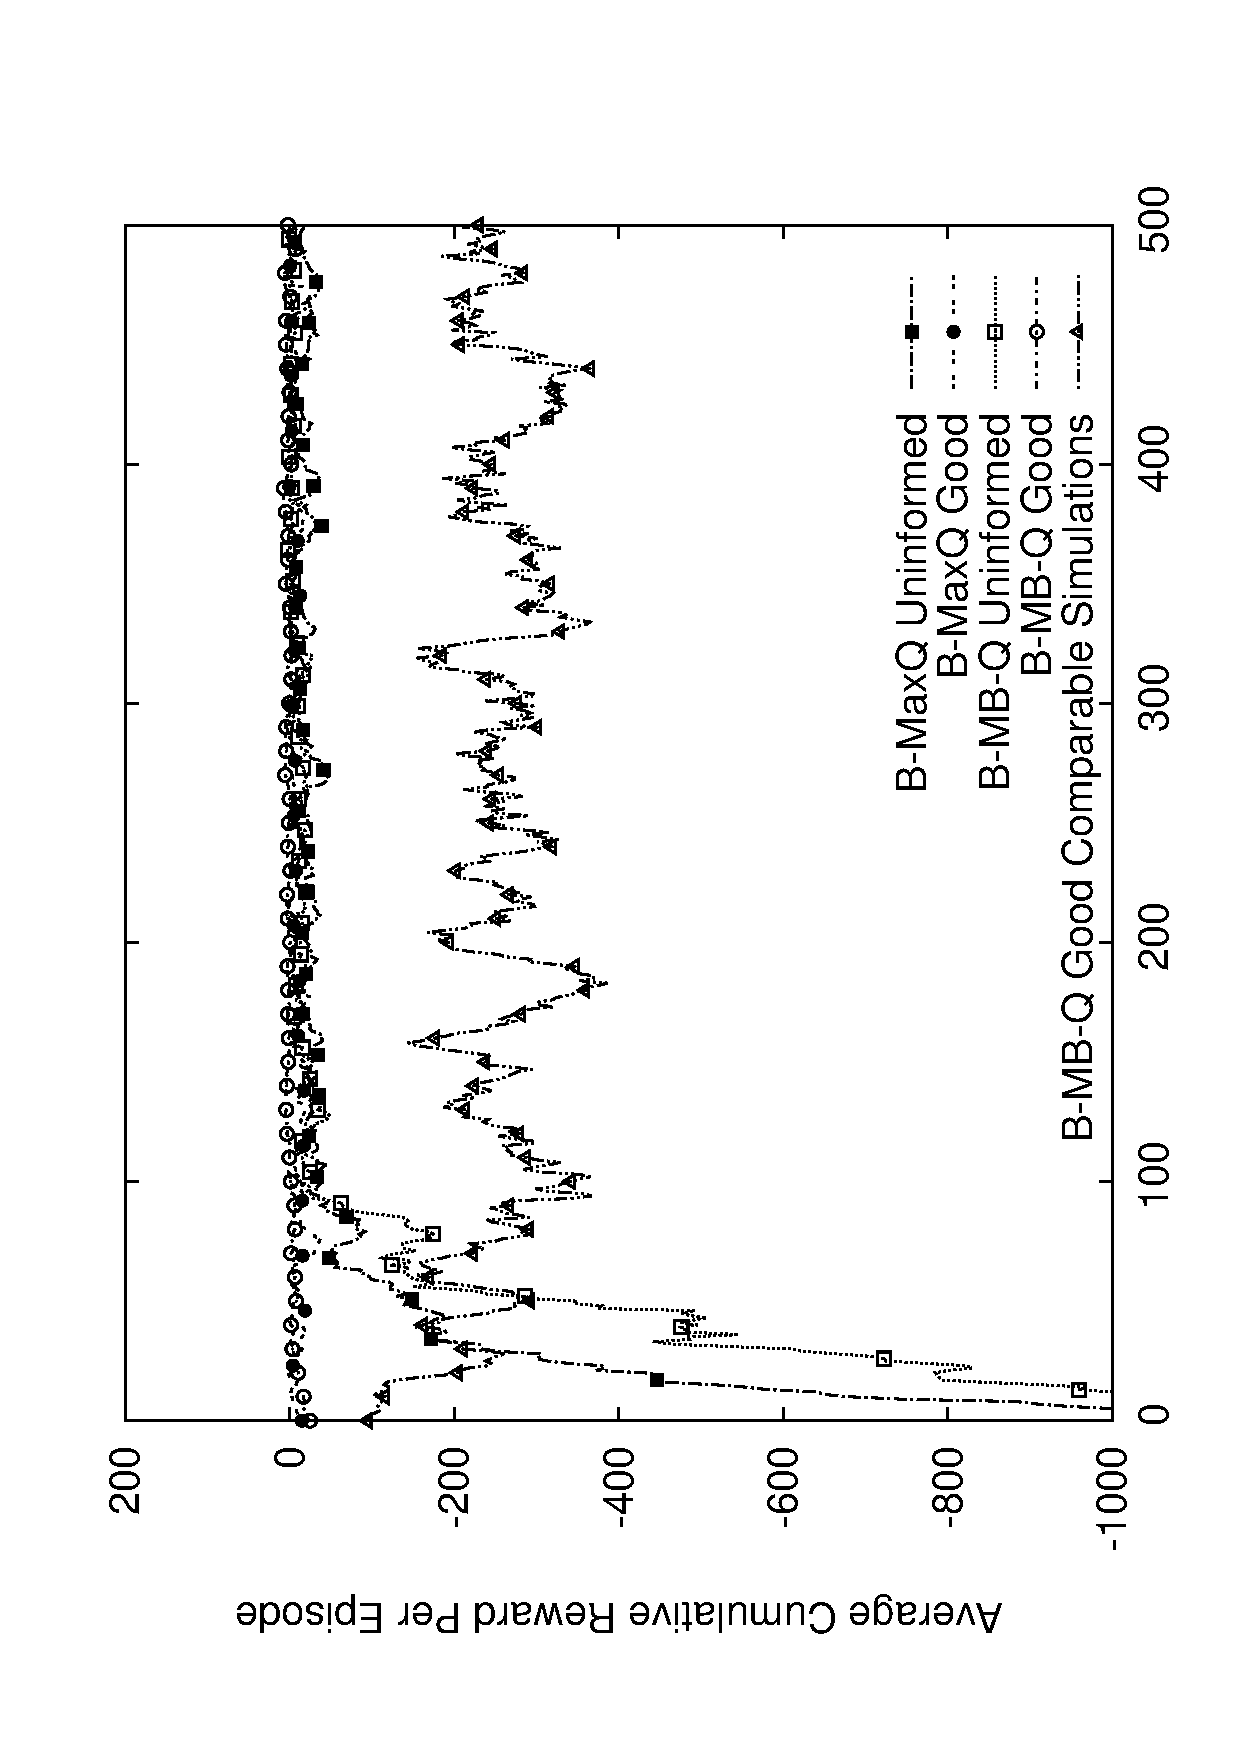
\includegraphics[trim=50 50 30 50, clip, scale=0.3]{exp/Taxib.pdf} & 
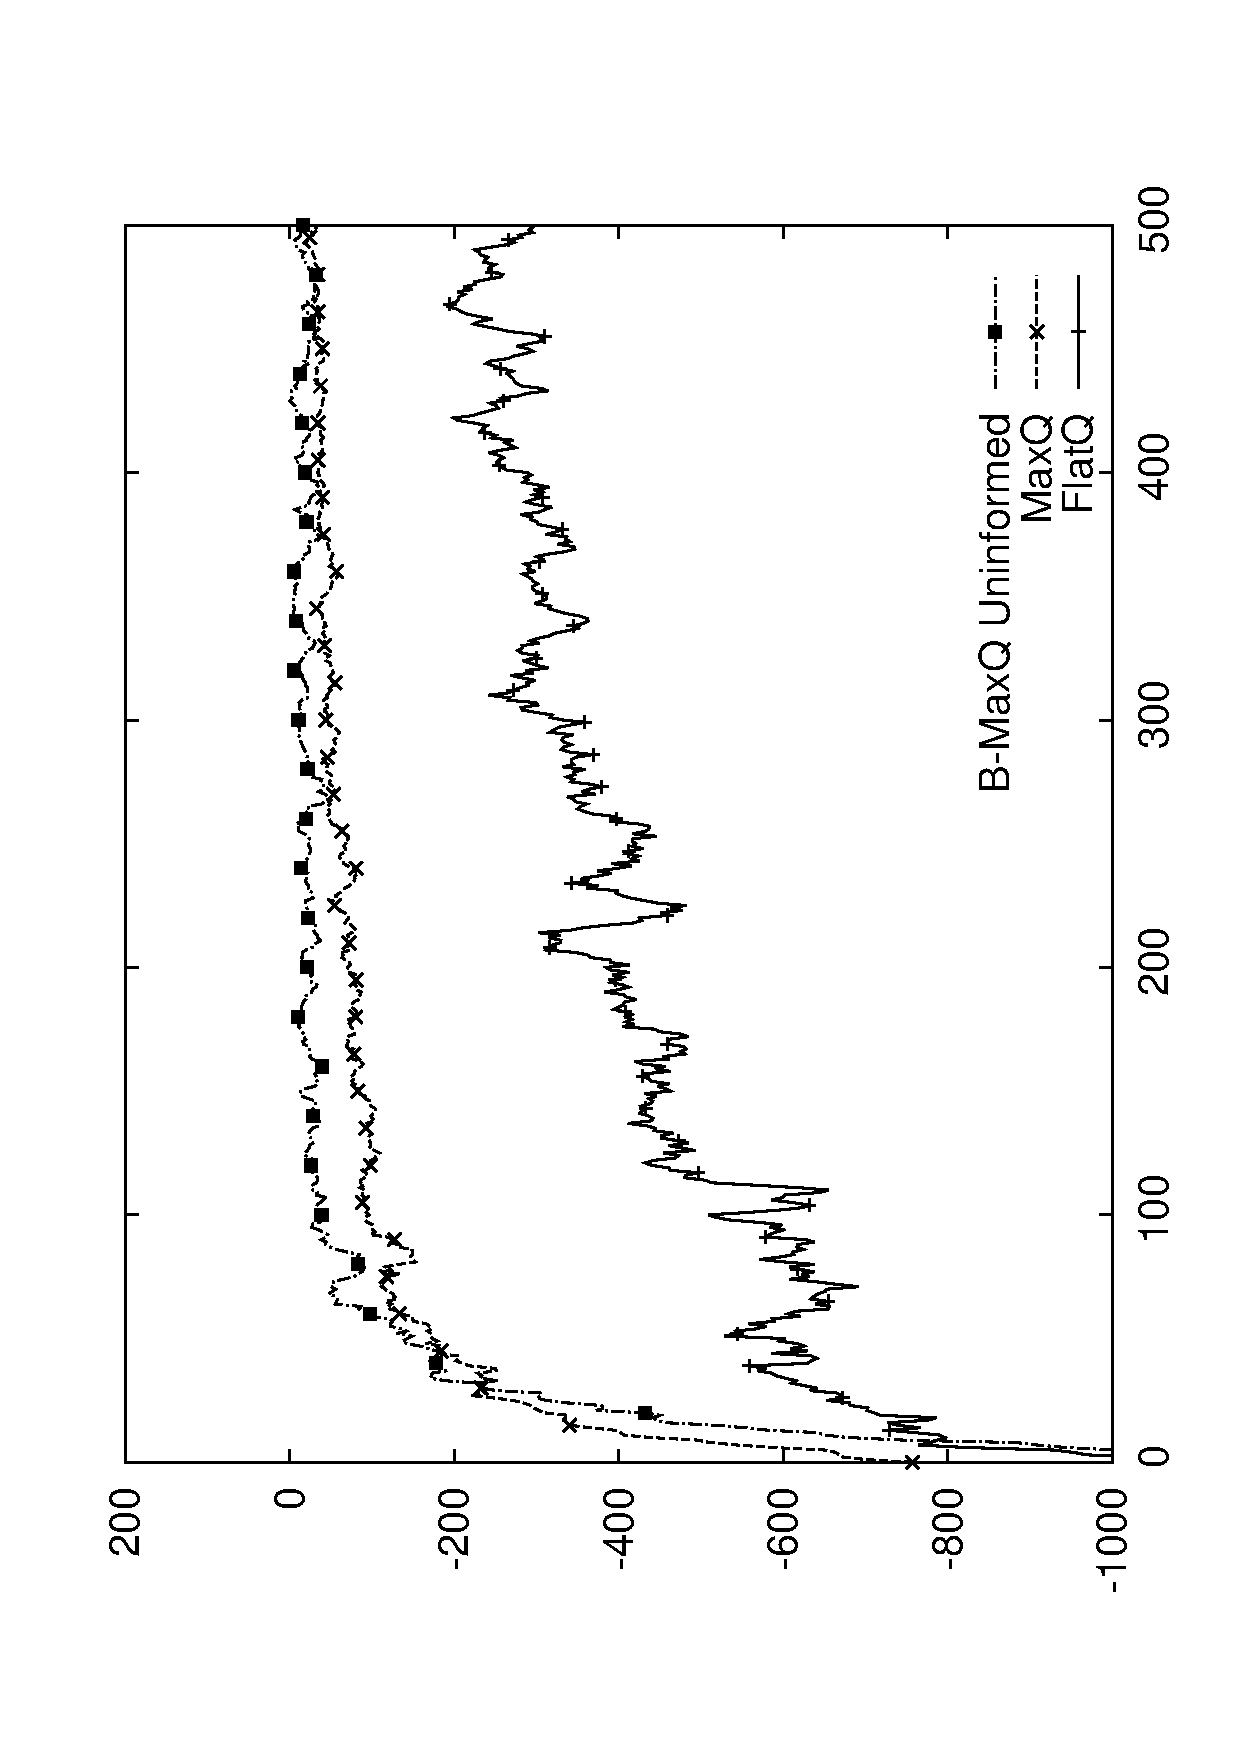
\includegraphics[trim=50 50 30 50, clip, scale=0.3]{exp/Taxinb.pdf} \\
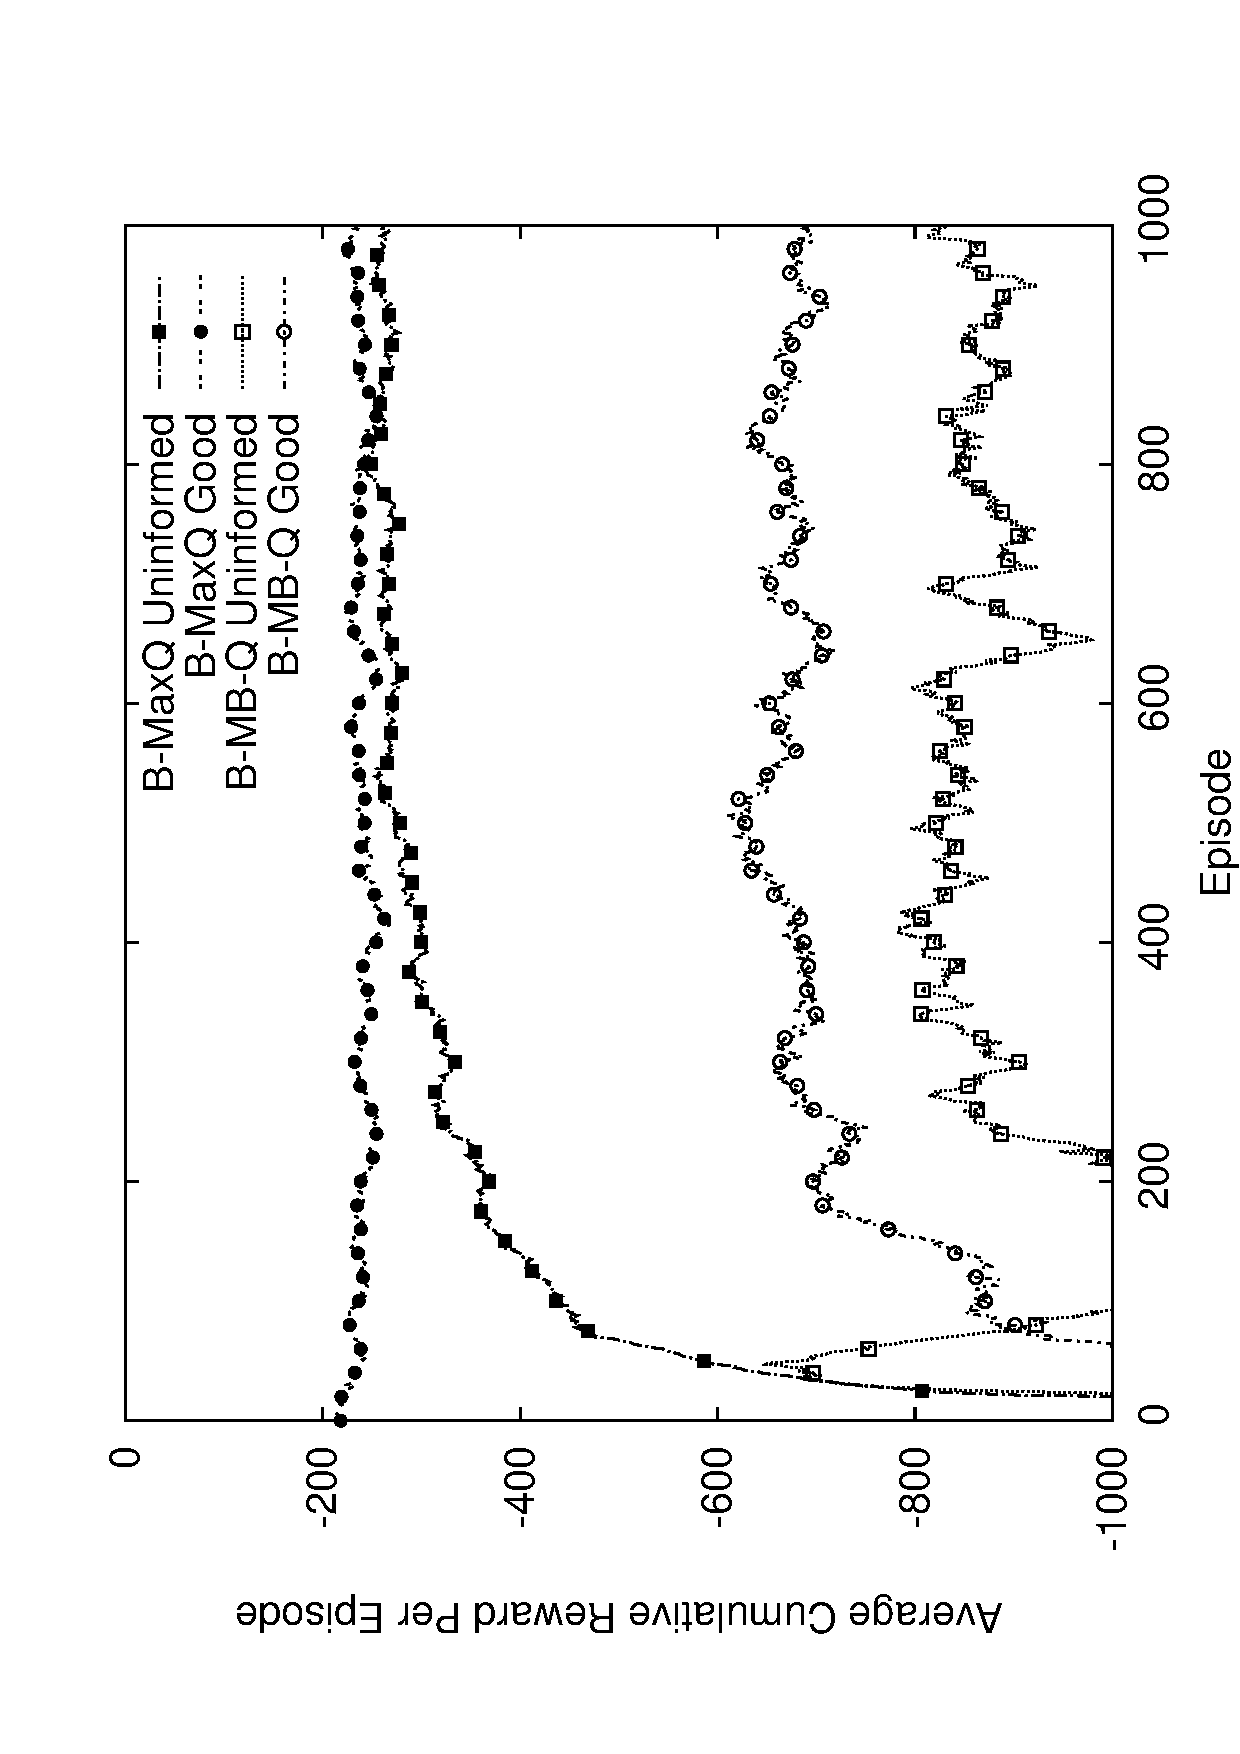
\includegraphics[trim=50 50 30 50, clip, scale=0.3]{exp/Wargus3322b.pdf} & 
\includegraphics[trim=50 50 30 50, clip, scale=0.3]{exp/Wargus3322nb.pdf} \\
\end{tabular}

%\vspace{-0.3in}
\caption{Performance of different algorithms on {\sf Taxi-World} (top row) and {\sf Resource-collection} (bottom row). The
prefix ``B-'' denotes Bayesian, ``Uninformed/Good'' denotes the
prior and ``MB'' denotes model-based.}\label{fig:nopr}
\vspace{-0.2in}
\end{figure*}

\section{Empirical Evaluation}
\label{sec:expts}

In this section, we evaluate our approach and test four hypotheses:
First, does incorporating model-based priors help speed up the
convergence of {\sc maxq} to the optimal policy? Second, how does the
task hierarchy interact with the prior? Does the task hierarchy still
matter if very good priors are available for primitive actions? Third,
how does Bayesian {\sc maxq} compare to standard (flat) Bayesian RL? Does
Bayesian RL perform better (in terms of computational time) if a task
hierarchy is available? Finally, can our approach effectively learn
pseudo-rewards and policies that are hierarchically optimal?
% \begin{figure}
% \begin{tabular}{cc}
% \hspace{-0.5in}\includegraphics[scale=0.4]{task/Taxi-Hierarchy.pdf}&
% \hspace{-0.5in}\includegraphics[scale=0.4]{task/Wargus-Hierarchy.pdf}\\
% \end{tabular}
% \caption{Task Hierarchies for {\sf Taxi-world} and {\sf Resource-collection}.}\label{fig:tasks}
% \vspace{-0.2in}
% \end{figure}

We first focus on evaluating the first three hypotheses using domains
where a zero pseudo-reward results in hierarchical optimality. To
evaluate these hypotheses, we use two domains: the 
fickle version of {\sf Taxi-World}~\cite{d-hrl-00} (625 states) and {\sf
  Resource-collection}~\cite{mehta.icml08} (8265 states). In {\sf Taxi-World}, the
agent controls a taxi in a grid-world that has to pick up a passenger
from a source location and drop them off at their destination. The
state variables consist of the location of the taxi and the source and
destination of the passenger. The actions available to the agent
consist of navigation actions and actions to pickup and putdown the
passenger.  The agent gets a reward of +20 upon completing the task, a
constant -1 reward for every action and a -10 penalty for an erroneous
action. Further, each navigation action has a 15\% chance of moving in
a direction orthogonal to the intended move. The {\sf
  Resource-collection} domain is inspired by real-time strategy games
where one component involves collecting resources from a map. We
simulate this through a grid world environment where the agent
controls a unit that can harvest gold and chop wood. Here the state
variables consist of the location of the agent, what the agent is
carrying, whether a goldmine or forest is adjacent to its current
location and whether a desired gold or wood quota has been met. The
actions available to the agent are to move to a specific location,
chop gold or harvest wood, and to deposit the item it is carrying (if
any). 
% To make the task tractable we limit the set of possible moves to
% a set of four locations adjacent to each goldmine, forest or deposit
% location. 
As before, for each navigation action the agent has a
probability of moving to a random location with 0.3 probability. 
% Further, in this
% domain, there may be multiple goldmines and multiple forests and
% multiple locations next to each goldmine and forest, so the action
% space is large. 
In our experiments, the map contains two
goldmines and two forests, each containing two units of gold and two
units of wood, and the gold and wood quota is set to three each. The
agent gets a +50 reward when it meets the gold/wood quota, a constant
-1 reward for every action and an additional -1 for erroneous actions
(such as trying to deposit when it is not carrying anything).
% The task hierarchies  are shown in
% Figure~\ref{fig:tasks}.

% \begin{figure*}[ht]
% \begin{tabular}{cc}
% %\hspace{-1in}\includegraphics[scale=0.6]{Taxi-Hierarchy.pdf} &
% %\hspace{-2.5in}\includegraphics[scale=0.6]{Wargus-Hierarchy.pdf}\\
% %\vspace{-5.2in}
% & \multirow{2}{*}{\includegraphics[scale=0.5]{task/Hallway-Hierarchy.pdf}} \\
% \includegraphics[scale=0.4]{task/Taxi-Hierarchy.pdf} & \\
% \includegraphics[scale=0.4]{task/Wargus-Hierarchy.pdf} & \\
% \end{tabular}
% \caption{Task Hierarchies for {\sf Taxi-world} (top-left), {\sf Resource-collection} (bottom-left) and {\sf Hallway} (right)\\
% Note that in subtasks Sniff and Back of Hallway, parameter $p$ is perpendicular to $r$, $(x, y)$ is the location of agent when Back is called.}\label{fig:tasks}
% \end{figure*}



For the Bayesian methods, we use Dirichlet priors for
the transition function parameters and Normal-Gamma priors for the
reward function parameters. We use two priors: an uninformed prior,
set to approximate a uniform distribution, and a ``good'' prior where
a previously computed model posterior is used as the ``prior.''
% priors. The first case is an uninformed prior. Here the priors
%  are set to approximate a uniform distribution over model
% parameters. The second case is a ``good'' prior. In this case, we
% first run the Bayesian MAXQ approach for 1000 episodes on each
% problem, and use the estimated model posterior as the prior.
 The prior
distributions we choose are conjugate to the likelihood, so we can compute the
posterior distributions over the relevant parameters in closed form.
In general, this is not necessary; more complex priors could be used
as long as we can sample from the posterior distribution.
\renewcommand{\arraystretch}{1}
\begin{table}[t] \footnotesize

\caption{CPU time for methods on {\sf Taxi-World}.}

\label{tab:time}

\begin{center}

\begin{tabular}{| p{4cm} | l |}

\hline

\multirow{3}{*}{Method} & Time for \\

&500 Episodes (s)\\ \hline

Bayesian MaxQ, Uninformed Prior &179\\ 

Bayesian Model-based Q, Uninformed Prior &232\\ 

Bayesian MaxQ, Good Prior &14\\ 

Bayesian Model-based Q, Good Prior &119\\ 

Bayesian Model-based Q, Good Prior \& Comparable Simulations
&934 \\ 

MaxQ &1.15 \\

FlatQ &0.53 \\
\hline
\end{tabular}

\end{center}
\vspace{-0.2in}
\end{table}

The methods we use in this experiment are: (i) Flat Q, the standard,
non-Bayesian Q-learning algorithm, (ii) {\sc maxq-0}, the standard,
non-Bayesian Q-learning algorithm for {\sc maxq} with no pseudo-reward,
(iii) Bayesian model-based Q-learning with an uninformed prior and (iv) a ``good'' prior, (v) Bayesian {\sc maxq} (our proposed approach) with
an uninformed prior and (vi) with a ``good'' prior. In our implementation,
the Bayesian model-based Q-learning uses the same code as the Bayesian
{\sc maxq} algorithm, with a ``trivial'' hierarchy consisting of the Root
task with only the primitive actions as children. For the Bayesian methods, the update frequency $k$
was set to 50 for {\sf Taxi-World} and 25 for {\sf
  Resource-collection}. $Sim$ was set to 200 for Bayesian {\sc maxq} for
{\sf Taxi-World} and 1000 for Bayesian model-based Q, and to 1000 for
both for {\sf Resource collection}.
% We make two changes
% to the Bayesian MAXQ algorithm for efficiency: first, we use ``all
% states updating''~\cite{d-hrl-00}, where the completion function is
% updated fro all states seen in the child task rather than just the
% exit. Second, in Line~\ref{line:sample} in {\sc Recompute\_value}, we
% sample a model from the posterior~\cite{Strens}. We observed that, as
% noted by others~\cite{icml2007}, the convergence behavior can be
% improved by sampling an approximately MAP model. We approximate this
% by computing the MAP model from our posterior, and then using an
% $\epsilon$-greedy hierarchical policy to select actions. 
The results
 are shown in Figure~\ref{fig:nopr}. 

From these results, comparing the Bayesian versions of {\sc maxq} to 
standard {\sc maxq}, we observe that for {\sf Taxi-World}, the
Bayesian version converges faster to the optimal policy even with the
uninformed prior, while for {\sf Resource-collection}, the convergence
rates are similar. When a good prior is available, convergence is
very fast (almost immediate) in both domains. Thus, the availability
of model priors can help speed up convergence in many cases for HRL.

Next, we compare the Bayesian {\sc maxq} approach to ``flat'' Bayesian
model-based Q learning. We note that in {\sf Taxi-World}, with uninformed
priors, though the ``flat'' method initially does worse, it soon
catches up to standard {\sc maxq} and then to Bayesian {\sc maxq}. This is
probably because in this domain, the primitive models are relatively
easy to acquire, and the task hierarchy provides no additional
leverage. For {\sf Resource-collection}, however, 
% Note that for the ``good'' prior in this task, Bayesian MAXQ
% and flat Bayesian model-based learning do about equally well. This
% indicates that in some cases the availability of a good model prior
% may reduce the need for a task hierarchy. However, this does not
% always happen, as shown in the {\sf Resource-collection} domain, where
even with a good prior, ``flat'' Bayesian model-based Q does not
converge. The difference is that in this case, the task hierarchy
encodes extra information that cannot be deduced just from the models.
In particular, the task hierarchy tells the agent that good policies
consist of gold/wood collection moves followed by deposit moves. Since
the reward structure in this domain is very sparse, it is difficult to
deduce this even if very good models are available. Taken together,
these results show that task hierarchies and model priors can be
complementary: in general, Bayesian {\sc maxq} outperforms both flat
Bayesian RL and {\sc maxq} (in speed of convergence, since here {\sc maxq} can
learn the optimal policy).

% Thus, good priors may not be sufficient to
% guarantee fast convergence---task hierarchies can encode additional
% information about good policies that help convergence even in the presence
% of good priors. However, if no such policy information is encoded by
% the hierarchy (e.g. the hierarchy allows all ``legal'' policies),
% then a good prior on the model reduces or eliminates the convergence advantage of
% HRL over flat RL.
\begin{figure}
\centerline{\includegraphics[scale=0.5]{task/Hallway-Hierarchy.pdf}}
\vspace{-0.3in}\caption{Task Hierarchy for {\sf Hallway}.}\label{fig:hallway}
\vspace{-0.2in}\end{figure}

\renewcommand{\arraystretch}{0}
\begin{figure*}[ht]
\centering
\begin{tabular}{cc}
\includegraphics[trim=50 50 30 50, clip, scale=0.3]{exp/Taxi_Modified_b.pdf} & 
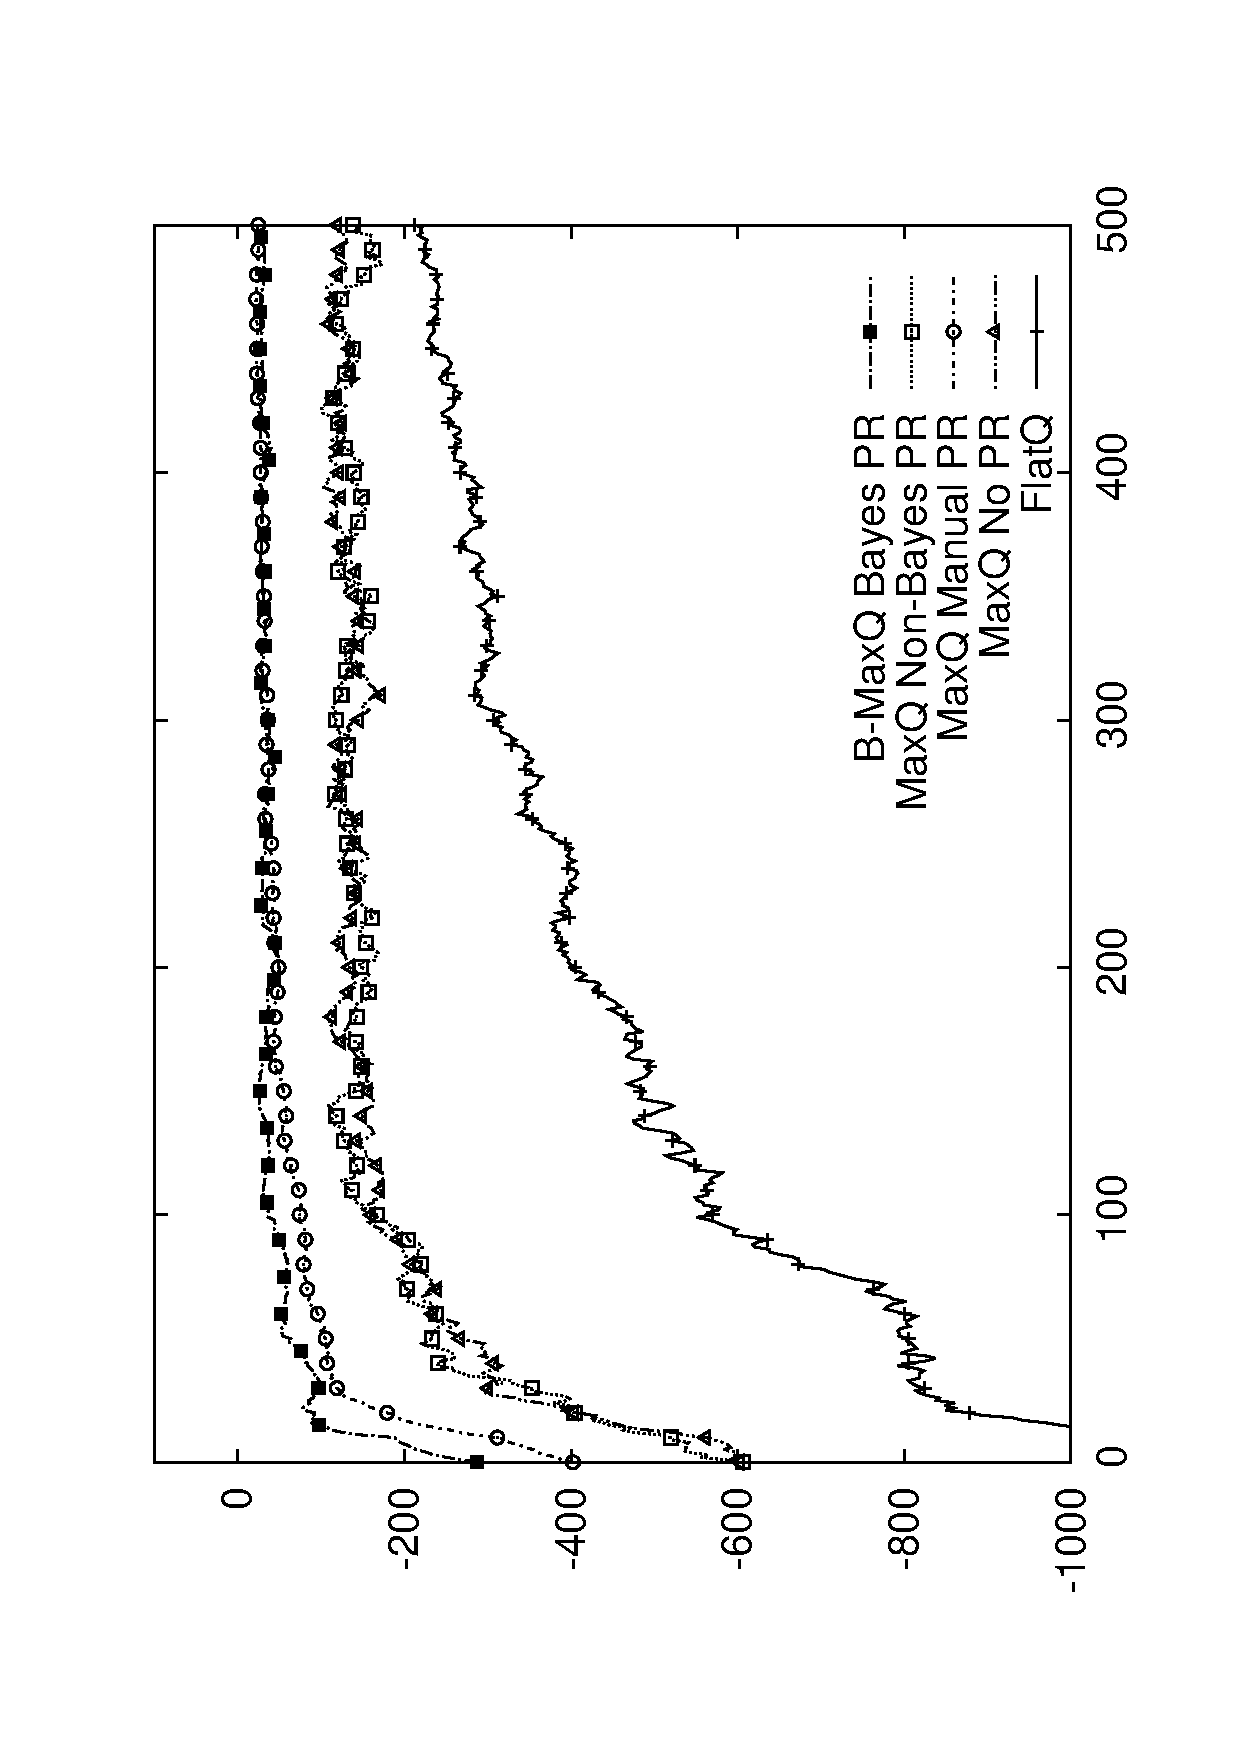
\includegraphics[trim=50 50 30 50, clip, scale=0.3]{exp/Taxi_Modified_nb.pdf} \\
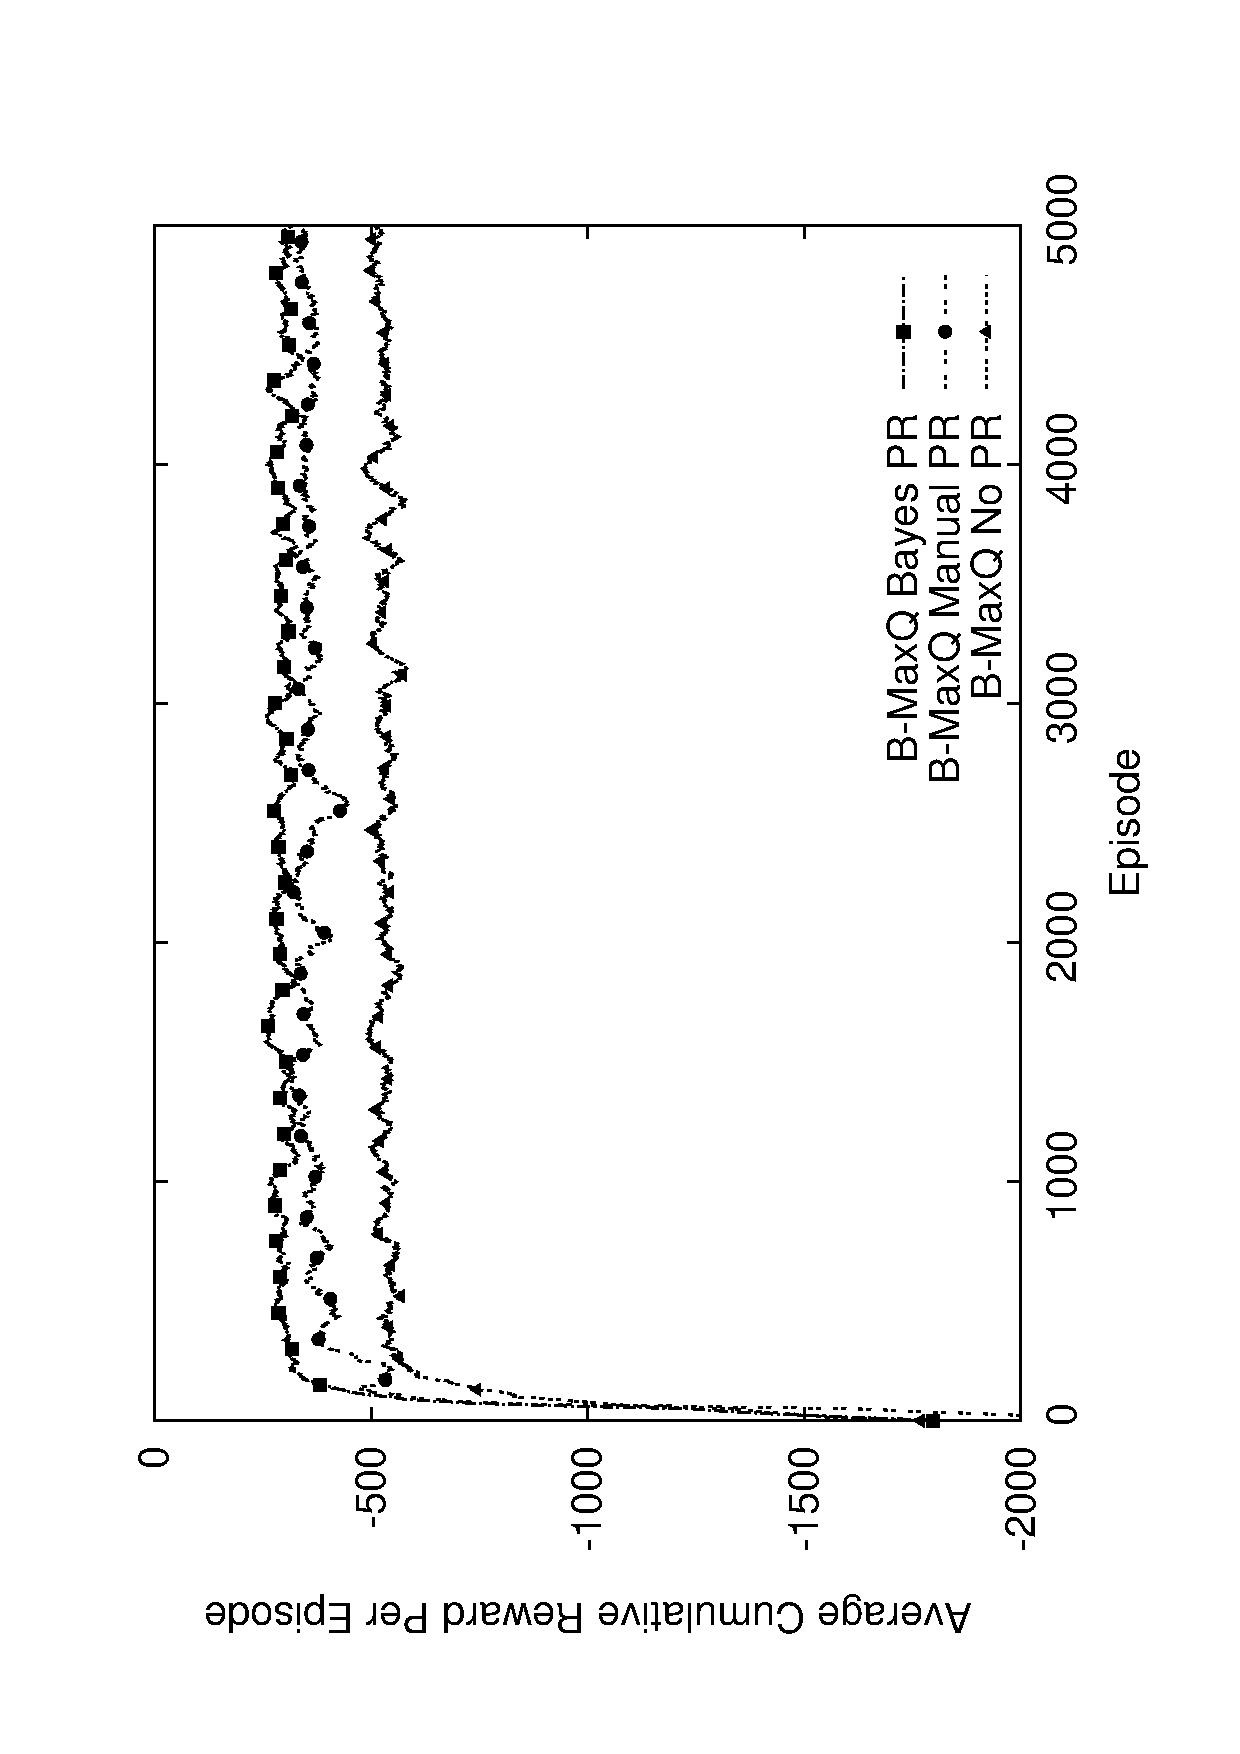
\includegraphics[trim=50 50 30 50, clip, scale=0.3]{exp/Hallwayb.pdf} & 
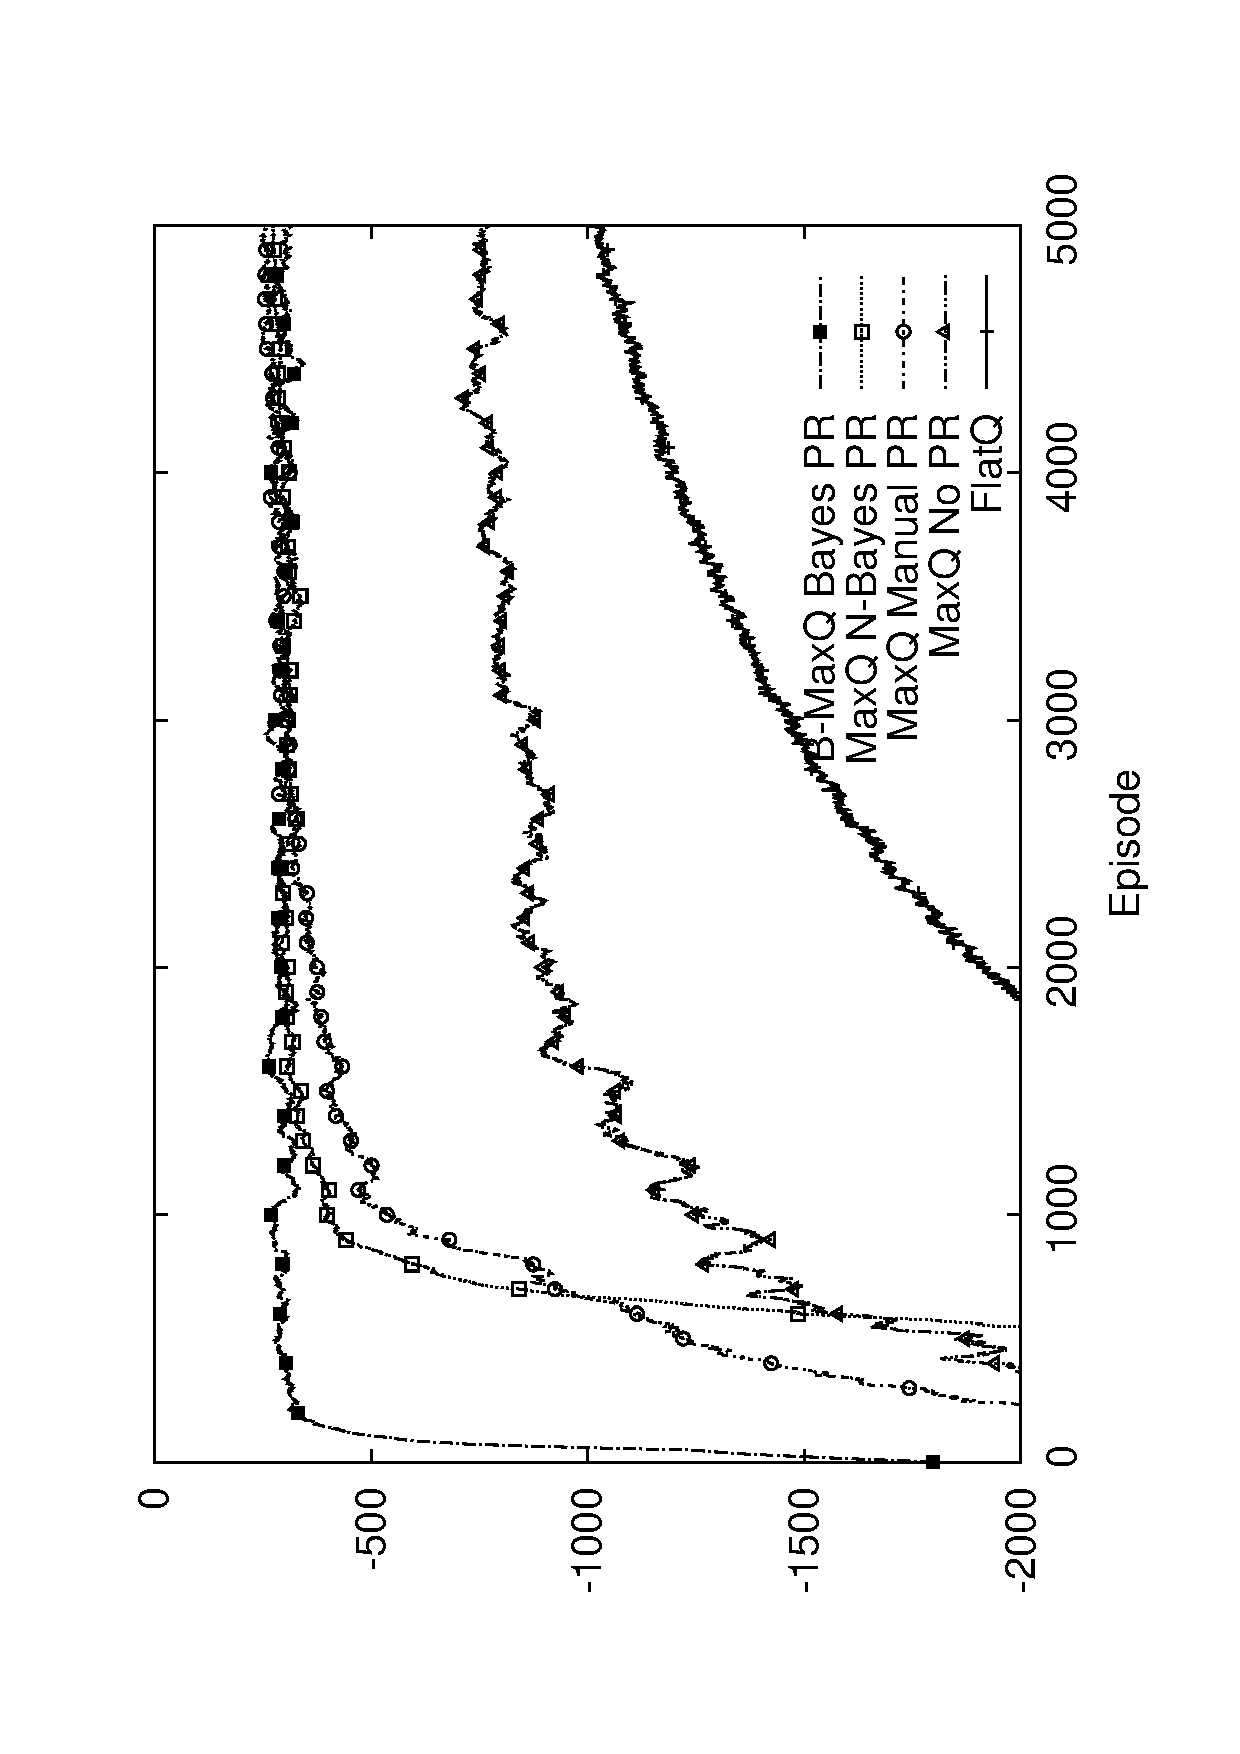
\includegraphics[trim=50 50 30 50, clip, scale=0.3]{exp/Hallwaynb.pdf} \\
\end{tabular}
%\vspace{-0.3in}
\caption{Performance of different algorithms on {\sf Modified-Taxi-World} (top row) and {\sf Hallway} (bottom row). The
prefix ``B-'' denotes Bayesian, ``PR'' denotes Pseudo Reward.}\label{fig:pr}
\vspace{-0.2in}\end{figure*}

Next, we compare the time taken by the different approaches in our
experiments in {\sf Taxi-World} (Table~\ref{tab:time}). As expected, the
Bayesian RL approaches are significantly slower than the non-Bayesian
approaches. However, out of the Bayesian methods, the Bayesian {\sc maxq} approaches are
significantly faster than the flat Bayesian model-based
approaches. This can be attributed to the fact that for the flat case,
during the simulation in {\sc Recompute\_value}, a much larger task
needs to be solved, while the Bayesian {\sc maxq} approach is able to take
into account the structure of the hierarchy to only simulate subtasks
as needed, which ends up being much more efficient. However, we note
that we allowed the flat Bayesian model-based approach 1000 episodes
of simulation as opposed to 200 for Bayesian {\sc maxq}. Clearly this
increases the time taken for the flat cases. But at the same time,
this is necessary: the ``Comparable Simulations'' row (and curve in
Figure~\ref{fig:nopr} top left) shows that, if the simulations are reduced to
250 episodes for this approach, the resulting values are no longer reliable and the performance of
the Bayesian flat approach drops sharply. Thus, taking advantage of
the hierarchical task decomposition helps reduce the computational cost of
Bayesian RL.


% \begin{table*}[t]
% \caption{CPU time taken by various methods on {\sf Taxi-world}.}
% \label{tab:time}
% \begin{center}
% \begin{tabular}{| p{4cm} | l | l | l | l | l |}
% \hline
% \multirow{5}{*}{Method} 	&Tot. Time  for	&\multicolumn{2}{|c|}{}  &\multicolumn{2}{|c|}{}			\\ 
% 						&500 Episodes 	&\multicolumn{2}{|c|}{Episodes with} 	 &\multicolumn{2}{|c|}{Episodes with}			\\
% 						&(s)				&\multicolumn{2}{|c|}{5-20 Steps}	&\multicolumn{2}{|c|}{70-120 Steps} 		\\ 
% 						&				&\multicolumn{2}{|c|}{(near-optimal)}		&\multicolumn{2}{|c|}{(suboptimal)}				\\ \cline{3-6}
% 						&
%                                                 &Avg Time (ms)	&Count
%                                                 &Avg Time (ms)	&Count \\ \hline
						
% Bayesian MaxQ, Uninformed Prior	&179	&21		&81 		&332  	&39 				\\ \hline
% Bayesian Model-based Q, Uninformed Prior	&232	&162 	&211 	&851	&25 					\\ \hline
% Bayesian MaxQ, Good Prior		&14		&17 		&209 	&84 		&3 				\\ \hline
% Bayesian Model-based Q, Good Prior		&119	&172 	&316 	&- 		&0 				\\ \hline
% Bayesian Model-based Q, Good Prior \& Comparable Simulations 									&934	&- 		&0		&687	&56		\\ \hline
% MaxQ							&0.53	&- 		&0		&1.49 	&171				\\ \hline
% Flat Q							&1.15	&- 		&0		&0.37	&18			\\ \hline
% \end{tabular}
% \end{center}
% \end{table*}



Finally we evaluate how well our approach estimates pseudo-rewards. Here we use two domains: a {\sf Modified-Taxi-World} and a
{\sf Hallway} domain~\cite{d-hrl-00,parr:thesis} (4320 states). In {\sf Modified-Taxi-World}, We allow dropoffs at any one of the four specific locations and do not provide a reward for task
termination. Thus the Navigate subtask needs a pseudo-reward
(corresponding to the correct dropoff location) to learn a good policy.
The {\sf Hallway} domain consists of a maze with a large scale
structure of hallways and intersections. The agent has stochastic movement actions. The task hierarchy is shown in Figure~\ref{fig:hallway}. 

For these experiments, we use uninformed priors on the
environment model. The pseudo-reward priors are set to prefer each
exit from a subtask equally. The baselines we
use are: (i) Bayesian {\sc maxq} and {\sc maxq} with fixed zero pseudo-reward, (ii)
Bayesian {\sc maxq} and {\sc maxq} with fixed manually set pseudo-reward, (iii)
flat Q and (iv) {\sc maxq} with a non-Bayesian pseudo-reward update. This last
method tracks pseudo-reward just as our approach; however, instead of
a Bayesian update, it updates the pseudo-reward using a temporal
difference update, treating it as a simple value function. The results
 are shown in Figure~\ref{fig:pr}.

From these results, we first observe that the methods with zero
pseudo-reward always do worse than those with ``proper'' pseudo-reward,
indicating that in these cases the recursively optimal policy is not
the hierarchically optimal policy. When a pseudo-reward is manually
set, in both domain, {\sc maxq} converges to better policies. We observe that
in each case, the Bayesian {\sc maxq} approach is able to learn a policy
that is as good, starting with no pseudo rewards; further, its
convergence rates are often better. Further, we observe
that the simple TD update strategy (MaxQ Non-Bayes PR in Figure~\ref{fig:pr}) fails in both cases---in {\sf Modified-Taxi-World}, it is able to learn a policy that is approximately as good
as a recursively optimal policy, but in the {\sf Hallway} domain, it
fails to converge completely, indicating that this strategy cannot
generally learn pseudo-rewards. These results indicate that a strategy
that incorporates Bayesian methods into {\sc maxq} can successfully learn
pseudo-rewards from scratch and produce hierarchically optimal policies.



%%%% Hallway Domain
%Parr illustrated his work using the maze shown in Figure 14. This maze has a large-scale
%structure (as a series of hallways and intersections), and a small-scale structure (a series of
%obstacles that must be avoided in order to move through the hallways and intersections).
%In each trial, the agent starts in the top left corner, and it must move to any state in the
%bottom right corner room. The agent has the usual four primitive actions, North, South,
%East, and West. The actions are stochastic: with probability 0.8, they succeed, but with
%probability 0.1 the action will move to the left and with probability 0.1 the action will
%move to the right instead (e.g., a North action will move east with probability 0.1 and
%west with probability 0.1). If an action would collide with a wall or an obstacle, it has no
%eect.
%The maze is structured as a series of rooms, each containing a 12-by-12 block of states
%(and various obstacles). Some rooms are parts of hallways, because they are connected
%to two other rooms on opposite sides. Other rooms are intersections, where two or more
%hallways meet.


\section{Conclusion}
\label{sec:conclusion}

In this paper, we have proposed an approach to incorporating
probabilistic priors on environment models and task pseudo-rewards
into HRL by extending the {\sc maxq} framework. 
%Our approach uses a
%combination of model-based and model-free learning to compute a
%hierarchically optimal policy. 
Our experiments indicate that several
synergies exist between HRL and Bayesian RL, and combining them is
fruitful. In future work, we plan to investigate approximate model and value representations, as well as multi-task RL to learn the priors.
%where models and value functions cannot be exactly represented, as well as investigate multi-task RL scenarios where the priors we currently assume to be given can be learned.

% priors can speedup convergence for HRL; (ii) however, good priors can
% reduce or eliminate the convergence advantage of HRL over flat RL, if
% the hierarchy does not encode ``strong'' policy constraints, and (iii)
% the cost of Bayesian RL can be reduced in the HRL setting, because the
% sampled solutions only involve subtasks rather than the whole task and
% so can be substantially more efficient. In future work, we propose to
% investigate methods to incorporate priors on value funcitons into the
% learning process, as well as investigate multi-task RL scenarios where
% the priors we currently assume to be given can be learned.


%\subsubsection*{Acknowledgments}
%
%Use unnumbered third level headings for the acknowledgments. All
%acknowledgments go at the end of the paper. Do not include 
%acknowledgments in the anonymized submission, only in the 
%final paper. 
%
%\subsubsection*{References}

\bibliographystyle{unsrt}
{\footnotesize
\bibliography{main}
}

\end{document}
